
%---------------------------------------------------------------------------------------------------------------------------------------------
\chapter{Notes}
\section{INTRO}
\subsection{History}
\subsection{bw1}
\section{LIT REVIEW}
finding a fuel optimal trajectory for a very-low-thrust power-limited lunar mission

gap: power limitation

\subsection{Past missions}
Need review of \cite{Herman1998}

need review of SMART-1 optimisation \cite{Schoenmaekers2004}

% Optimisation methods
\subsection{Optimisation methods}
\textcite{McKay2011} provide a survey of non-keplerian orbits, which they define as any orbit with forces additional to the primary point-mass gravitational force. Their study was focussed towards using low thrust propulsion to maintain a stable orbit in the presence of these secondary forces, and while \BW\ requires a transfer trajectory rather than a stable orbit their paper does conclude that there are some serious deficiencies with established research in the area:
\enquote{It is clear, however, that work still has to be done to transform the steadily growing body of literature on highly-non-Keplerian orbits from interesting theory into actual, practical missions.} 

evolutionary algorithms often need distributed computing environments due to the number of computations involved \textcite{Lee2005}

genetic algorithms and simulated annealing \textcite{Lee2005}

Pareto-optimality based on the economic theory by Italian Vilfredo Pareto, implying that it is the best solution that can be found without compromising other objectives, in this case the best fuel efficiency that can be found without taking an unreasonable amount of time. \parencite{Lee2005, Coverstone2000}

\textcite{Enright1992} hermite simpson/RK integration, direct shooting/multiple shooting/collocation, concludes -- direct transcription, NLP, \enquote{parallel shooting} RK
\begin{enumerate}
\item future work - lower thrust levels, lower initial and final orbits, non-coplanar transfers
\item size of problem - much better mesh distribution, exploit sparsity
\item lunar eccentricity and better geopotential do not affect problem size (just time to solve; longer computation each step, but doesn't increase the number of steps).
\end{enumerate}

Pierson \& Kluever optimised Earth escape, backwards propagation for Moon \enquote{capture} to maximise lunar energy after a given time, with a cruise phase in between.

Comparison of retrograde and posigrade terminal orbits. Posigrade gives better performance.

Very minimal improvement on initial guess suggests optimisation method ineffective.

\enquote{Hybrid} direct/indirect approach.

100,000~kg and 2942~N. What kind of electric propulsion?! And are they suggesting sending the ISS to lunar orbit?!

Uses SQP to solve 2PBVP

Melbourne and Sauer - Mars trajectories under solar gravity only

Breakwell and Rauch - patched two-body trajectories

Not much work on reduced three-body problem

London and Stuhlinger - patched two-body segments

Golan and Breakwell - variable thrust magnitude trajectories with no coasting arcs

Enright and conway - collocation, determining a single minimum fuel, low thrust, earth-moon transfer.

\textcite{Kluever1996} outlines his experimental procedure to find an initial guess: simulate under thrust, modifying phase time until near SOI. Then simulate for 7-8 days to observe the lunar fly-by, adjusting initial angle (in a 2D moon-fixed frame) until coasting trajectory enters SOI with negative moon-relative radial velocity component. Backwards propagate the lunar descent, adjusting phase length until the orbital energy is about the same as the end of the coasting arc.

Citing other peoples' graphs in Lit Review: .... Reproduced from \cite{}

\textcite{Kluever1997} extends the work to 3D, even includes a polar lunar orbit. Still starting from very high earth orbit, still much higher thrust. Uses direct optimisation but pontryagin necessary conditions to parameterise the intial guess control profile.

Initial guess based on 2D optimisations for GEO-HLO. Optimisation slowly converts plane change from HLO-LLO phase  until it is almost entirely included in GEO-HLO phase.

T/W ratio of 1.3e-4

\textcite{Kluever1995} assumes initial LEO in lunar plane.

All constant thrust, constant mass flow, giant spacecraft, does not address initial launch (inclination, capability to launch that mass). Due to simplifications like no external forces and constant thrust, the inverse costate equations were found allowing the Pontryagin principle to be exploited in order to get a very accurate initial guess for the thrust profiles in ascent and descent phases. SQP is then used to blend the phases together.

% ------------------------------------------------ MODELLING ------------------------------------------------
\section{MODELLING}
\subsection{Time}
\subsection{Reference frames}
model keplerian coordinates diagram on \cite{Pollard2000}

explanation of LCI frame - see \cite{Erb_thesis}

\subsection{Coordinate systems}
local orbit coordinates: LVLH (local vertical - radial x direction; local horizontal - tangent) also known as the Gauss frame. \cite{STK}

define LCI, SEL, ECI

\subsection{Orbital elements}
\subsection{Equations of motion}
\subsection{Perturbations}
Earth harmonics affect mostly $\omega$ and $\Omega$ - witness SSO, precess 360\degrees\ per year due to harmonics but minimal inclination change.

earth harmonics affect $\omega$ and $\Omega$ mostly. \textcite{Eshagh2007} 

SSO inclination doesn't change (only need to model J2)

GEO needs J4

oblateness causes small periodic deviations, only RAAN and arg. of periapsis are subject to long term change \textcite{Montenbruck2000}

\subsection{Figures of merit}
\begin{equation}
\Delta v= c_{PPT}\ln\frac{m_4}{m_3}+c_{arcjet}\ln\frac{m_3}{m_2}+c_{PPT}\ln\frac{m_2}{m_1}+c_{arcjet}\ln\frac{m_1}{m_0}
\end{equation}

\subsection{Other factors}
Space debris

Radiation - hardened hardware

Explain van Allen Belts? Picture in earlier sections as per Falke and Letterio theses
\begin{figure}
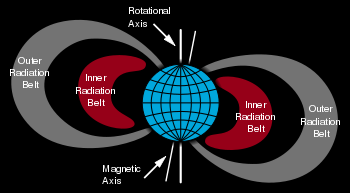
\includegraphics[width=\textwidth]{Images/350px-Van_Allen_radiation_belt_svg.png}
\caption{The van Allen Belts conceptual image}\label{fig:vabs}
\end{figure}
outer radiation belt extends from an altitude of about three to ten Earth radii, and is characterised by a relatively high density of high energy (0.1-10~MeV) electrons trapped within Earth's magnetosphere. The density varies wildly based on geomagnetic storms and variations in solar wind.
much more worrying is the inner belt which extends from an altitude of 100~km (the edge of space) to about 10,000~km, and consists of high concentrations of energetic protons (some over 400~MeV, which can penetrate 143~mm of lead) thought to be caused by cosmic ray collisions with nuclei of the upper atmosphere.
\begin{figure}
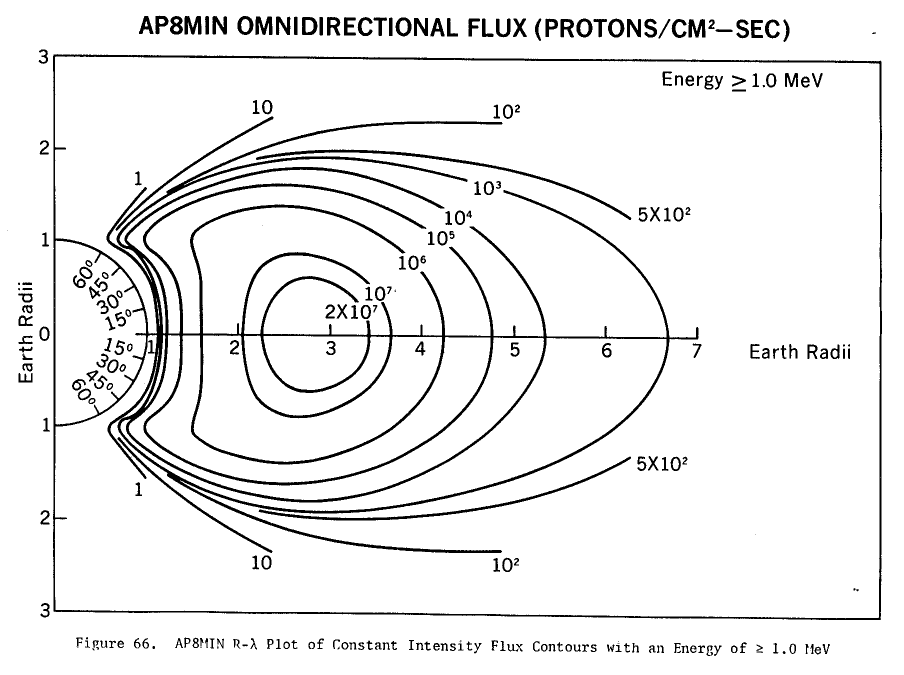
\includegraphics[width=\textwidth]{Images/Ap8-omni-1_000MeV.png}
\caption{The van Allen Belts proton flux distribution \parencite{Sawyer1976}.}\label{fig:vabs}
\end{figure}

reaction wheels for attitude control; at the moment no external thrusters for attitude control. It has been suggested to use the PPTs for reaction wheel desaturation, although they can only remove pitch and yaw, not roll.

% ------------------------------------------------ OPTIMISATION ------------------------------------------------
\section{OPTIMISATION}
\subsection{Formulation}
\subsection{State vector}
\subsection{Independent parameter}
\subsection{Objective function}
fixed launch mass at initial guess because that is how it is booked with launch service provider. saving fuel means more scientific payload.

choice of objective function and bounds for cruise phase - computational difficulties due to it being captured by moon (and therefore retrograde relative to earth) or escaping earth and losing dependence on L. Therefore put path constraint that it does not escape earth, and terminal constraint that it is not closer to escaping than the Moon is. Objective function is orbital energy wrt Moon to ensure capture, scaled by magnitude of energy last orbit so that it does not drown out fuel objective.

mention that Erb used lower limit on lunar energy to prevent it dropping too far into lunar orbit, and limit on eccentricity (although he was aiming for an eccentric final orbit). Then used objective function of minimising orbital energy and eccentricity, for the counter-intuitive approach of putting a limit on the parameters you are trying to optimise. This scenario becomes a delicate balancing act between the two variables, based on the arbitrary weightings given to them in the cost function.

\subsection{bvp}
initial arg of periapsis and RAAN depend on time of launch

\subsection{Simulation}
propagatephase with tangential thrust profile to get approximate $\Delta L$ required, use that as initial guess in optimisation.

\subsection{Optimisation}
From Wiki (paraphrased):
there are two categories of techniques used to solve trajectory optimisation problems: indirect methods, that rely on the inverse equations of motion to determine the gradient at a given point (and determine a local optimum to exist where the gradient is zero) and direct methods that simply find a point with a better objective function than any adjacent points.

The optimal control problem is an infinite dimensional problem (since a continuous control profile provides an infinite amount of variability). 

Can be solved by a number of analytical methods, but these often require extensive approximations and assumptions.
\enquote{An example is given in \textcite{Ohlmeyer2006}. In this example, linear assumptions are made and yet the algorithm can produce near optimal trajectories. Another example of an analytic solution is the \enquote{Iterative Guidance Mode (IGM)}, the guidance algorithm used by the two exo-atmospheric stages of the Saturn V rocket. The IGM algorithm is an analytical calculus-of-variations solution of the two-point boundary value problem posed by the ascent of the rocket to prescribed orbit-injection conditions.}

The dimensional complexity can be reduced by discretising it into a high-order numerical problem (typically with hundreds or thousands of degrees of freedom). Numerical algorithms are then used to estimate the gradient (the Jacobian matrix) of the objective function for a given solution, to find the direction to adjust optimisable parameters to improve the value of the objective function.

Second-order methods are also available to improve the rate of convergence, for example, the Newton–Raphson iteration, which requires the evaluation of the Hessian matrix (the second order gradient matrix). 

These techniques are collectively known as \enquote{numerical optimal control}. The disadvantage of numerical optimal control is that the Jacobian and Hessian matrices can be very difficult (sometimes impossible) to determine.

Consequently an alternative method was developed, relying on direct optimisation methods to circumvent these difficult calculations. 

Collectively known as \enquote{non-linear programming}, these techniques approximate the problem by a finite dimensional problem.

NLP techniques, such as the Broyden–Fletcher–Goldfarb–Shanno (BFGS) method and Sequential Quadratic Programming (SQP)

From Wiki?:
\enquote{As computation time has become cheap compared to manpower, direct sample methods have evolved as the optimization algorithms of choice. These algorithms may require orders of magnitude increases in the number of functional samples but exhibit robustness to non-smoothness in the trajectory code. Examples include: genetic algorithms\parencite{Hughes2004,Vasile2009}, stochastic sampling methods, and hill climbing algorithms. An overview of the state of the art in numerical methods is given in \textcite{Betts1998}.}

\cite{Betts2002}

\textcite{SOCS_guide}

\textcite{ASTOS_guide}

Hill-climbing... generic name for methods that get a solution, cast around for better objective function, then move on. But is SOCS truly this direct? Seems to compute Hessian and Lagrangian, albeit locally.

can perhaps use \cite{Well2001} for reference about GESOP, SQP, collocation, direct shooting

\cite{Hargraves1987} for a simple run-down on what direct optimisation is, with NLP and collocation

\textcite{Enright1992} outline of calculus of variations (indirect) vs. NLP (direct)

the optimal control problem is replaced with an approximate non-linear programming problem with the continuous control history replaced with a finite number of parameters.

\subsection{Numerical considerations}
normalisation / scaling of constraints - show output graphs, path constraints up to 200 (due to being many times the minimum distance from the earth) but better than $1.0\times10^8$~m 

real workspace size is measured in doubles (8~Bytes each) and integer workspace size is measured in longs (4~Bytes each), so numerical accuracy for doubles is 64~bits, with 53~bits of significand precision. Also, 1.6e8 doubles required for Cruise phase 1220~MB RAM, and 0.8e8 longs required, 305~MB RAM.

\subsection{Gesop}

\section{To be sorted}

Copy new sections from IAC paper 2010 \textcite{Shimmin2010}

\begin{enumerate}
\item Rewrite 1.1 outline
\item 2 what i have achieved (gap)
\item 2.5 Scope
\item 3.3 Optimisation methods and pictures
\item 4 corel draw for coordinate diagrams
\end{enumerate}

give ground access times from STK

\enquote{While the lunar orbit in DE 421 is close to that in DE 418, it is a major improvement over the widely distributed DE 405 (Standish 1998). For DE 405 the lunar orbit was not fit in a way consistent with the other planets}\cite{DE421}.

Ephemeris Time, used by the \textcite{NAIF2010}. Number of seconds since J2000 epoch.


ITRF - international terrestrial reference frame \url{http://itrf.ensg.ign.fr/} for oblateness

Lunar reference frames \url{http://naif.jpl.nasa.gov/naif/lunar_kernels.txt} \textcite{LCF}.

third body forces from Jupiter barycenter

The geographic parameters of satellite radius $r$, longitude $\lambda$ and latitude $\phi$ are calculated by converting the ECI frame to a body-fixed frame. The conversion is provided by the International Earth Rotation Service \parencite{Petit2010}.

Define J2000 frame and epoch

The IERS Celestial Reference Frame (ICRF) is offset from the J2000 reference frame (equivalent to EME 2000) by a small rotation:  the J2000 pole offset magnitude is about 18 milliarcseconds (mas) and the equinox offset magnitude is approximately 78 milliarcseconds (see [3]). \url{http://naif.jpl.nasa.gov/pub/naif/GRAIL/kernels/fk/moon_080317.tf}

The ITRF93 high accuracy Earth rotation model takes into account:
\begin{itemize}
\item Precession: 1976 IAU model due to Lieske.
\item  Nutation: 1980 IAU model, with IERS corrections due to Herring et al.
\item  True sidereal time using accurate values of TAI-UT1
\item  Polar motion
\end{itemize}



backwards propagation allows optimisation of mass - once final dry mass is known, can propagate backwards to determine how much wet mass is required.


\cite{Yam2011} attempts global search using basin hopping and simulated annealing, each hybridized with a local search algorithm. Has to approximate the low thrust maneouvre as a series of impulsive maneouvers.
cartesian state
theoretical nuclear electric mission to Jupiter, 2.26~N, 6000~s, 20000~kg with gravitational swing-bys.
another one to Mercury, 1300~kg, 0.34~N and 3200~s.


homotopy/embedding/continuation methods: optimise a simplified case (two body problem), then use that solution as the initial guess for a more sophisticated case, etc.


direct transcription
\begin{gather}
n \approx (n_y + n_u)MN
n_y = 8
n_u = 4
M = 4 optimisable phases
N = 80,000 grid points per phase
=2.56e6
\end{gather}
\cite{Betts1998}

SOCS implements a sparse SQP method based on a Schur-complement algorithm suggested by Gill et al. (Stanford technical papers)
Jacobian and Hessian matrices are computed efficiently using sparse finite differencing as proposed by Coleman1983 SIAM journal of numerical analysis and Curtis1974 Journal of the Institute of Mathematics and Applications

\section{SOCS output}
No DOF : number of parameters minus active constraints. Approx 50,000 for Cruise phase
Cond KKT system: condition number of Hessian matrix of Lagrangian, from Newton's method: $A\vec{x}=\vec{b}$ where $A$ is the Hessian, $\vec{x}$ is the system and $\vec{b}$ represents the perturbations. A high condition number means the system is highly sensitive to small changes in the perturbation vector. Approx 1e11

SOCS uses BFGS quasi-Netwon method to approximate Hessian (Broyden, Fletcher, Goldfarb, Schanno).

Cruise with NASA libraries: 200000000 doubles and 80000000 words
1e-4 opt tolerance, 1e-5 constraint tolerance, 2e-5 ODE tolerance